\documentclass[fleqn]{exam}

\usepackage{fullpage}
\usepackage{enumerate}
\usepackage{unitsdef} 
\usepackage{graphicx}
\usepackage[fleqn]{mathtools}
\usepackage{cancel}
\usepackage{polynom}
\usepackage{float}
\usepackage{mdwlist}
\usepackage{booktabs}
\usepackage{cancel}
\usepackage{polynom}
\usepackage{caption}

\setlength{\mathindent}{.5 cm}

\everymath{\displaystyle}

% \begin{figure}[H]
%   \centering
%   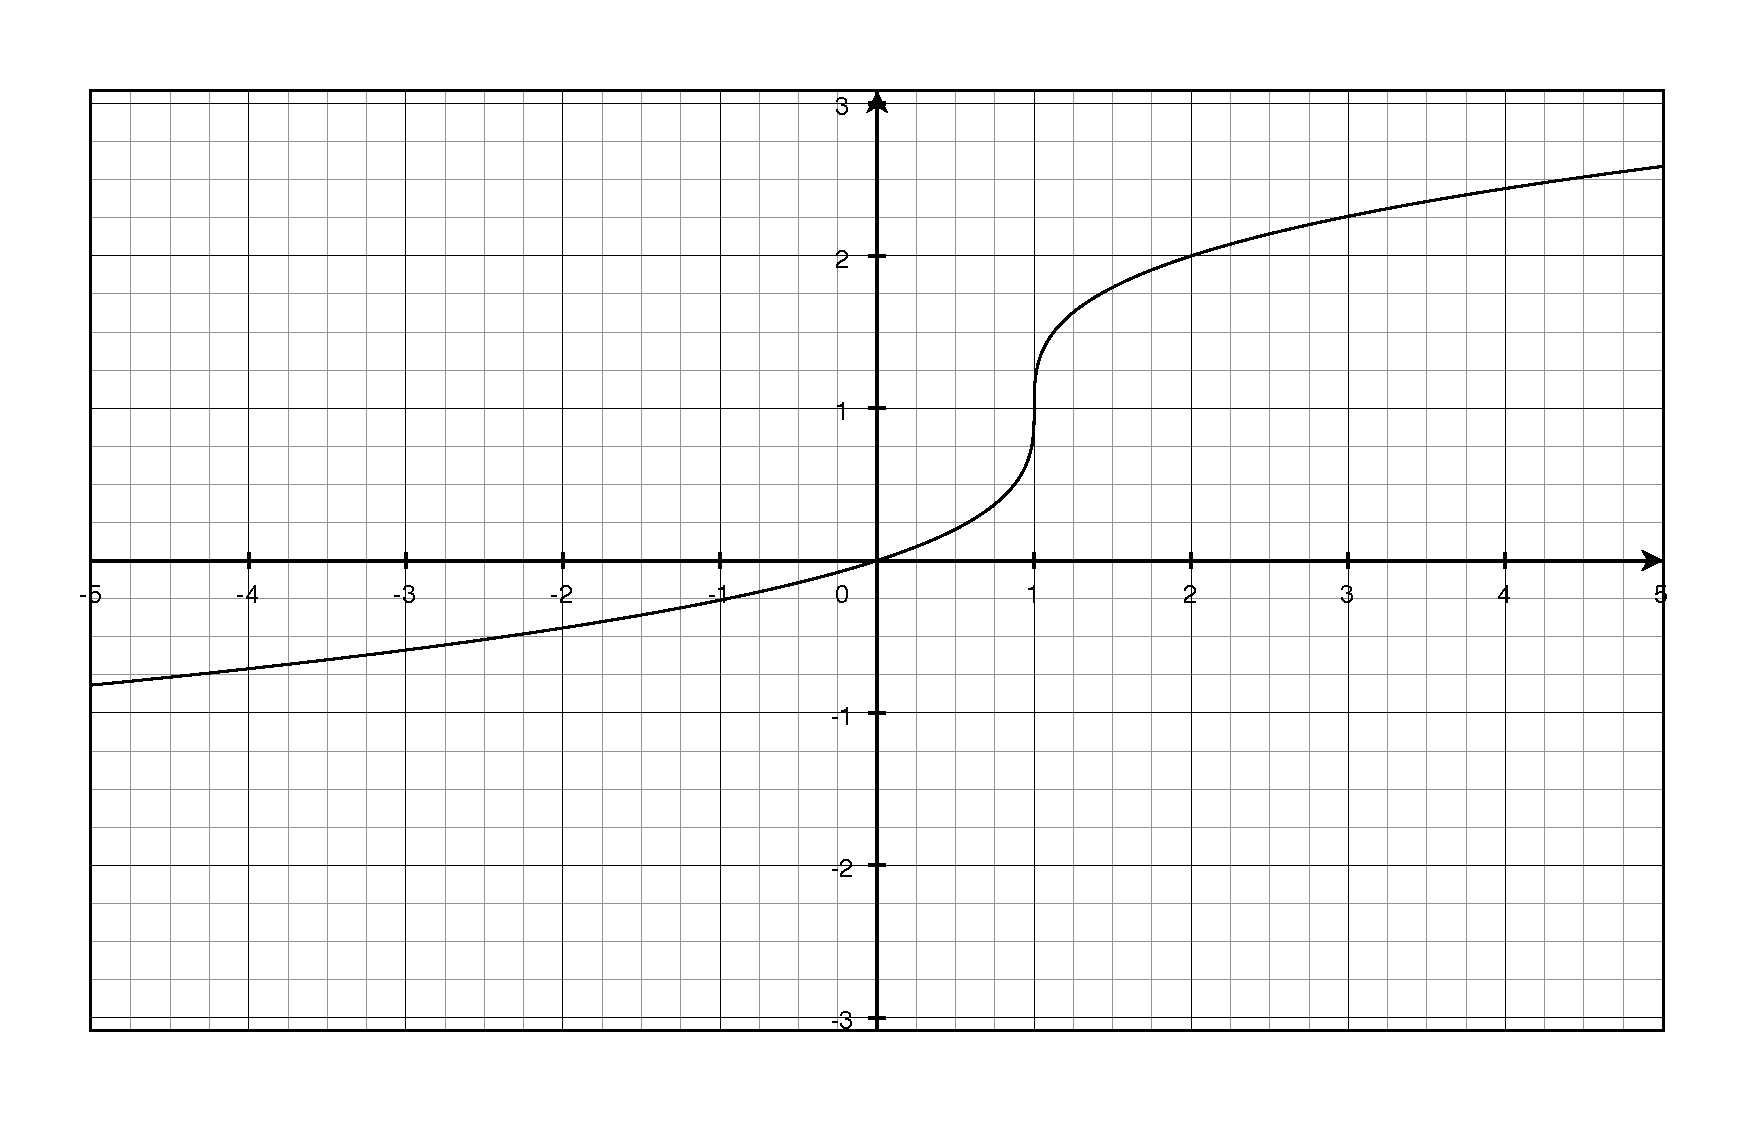
\includegraphics[scale=.3]{question7.eps}
%   \caption*{Question 7}
% \end{figure}

% \begin{tabular}{cc}
% \toprule
% period & amplitude \\
% \midrule
%   $\pi$ & $2$ \\
% \bottomrule
% \end{tabular}

\newunit{\inch}{in}
\newunit{\mile}{mile}
\newunit{\foot}{ft}
\newunit{\knot}{knot}
\newunit{\gallon}{gallon}

\printanswers

\ifprintanswers 
\usepackage{2in1, lscape} 
\fi

\title{Math 263A \\ Homework 14}
\date{May 9, 2012}

\begin{document}

\maketitle

\section{Homework}

\begin{itemize*}
  \item Read Section 4.3-4.4
  \item pp. 192-193: 1-4, 10-14, 20
  \item pp. 198-200: 1-2, 5, 7-9, 13-14, 16-17, 23
\end{itemize*}

\section{Extra Credit}
\begin{itemize*}
  \item page 192, problem 25
\begin{solution}
\begin{enumerate}[a]

\item $f$ is increasing whenever the derivative is positive: 

\begin{tabular}{ll}
\toprule
increasing & $(-\infty, -3] \cup [-1, 0)$ \\
decreasing & $[-3, -1] \cup (0, \infty)$ \\
\bottomrule
\end{tabular}

\item $f$ is concave up when $f'$ is increasing: .  It's concave down the rest of the time:

\begin{tabular}{ll}
\toprule
concave up   & $(-2, 0) \cup (0, 2)$ \\
concave down & $(-\infty, -2) \cup (2, \infty)$ \\
\bottomrule
\end{tabular}

\item $f'$ is 0 at $x = \{-3, -1, 2 \}$.  From parts b, $-3$ is a local maximum and $-1$ is a local minimum.  $f'$ is
  undefined at $x = 0$, but negative when $x < 0$ and positive when $x > 0$, so $0$ is a local maximum.

$f''(2) = 0$, so the second derivative test doesn't help for this point.  But $f'(x) < 0$ on both sides of this point so
  it is neither a local minimum or a local maximum.

\item The inflections points are when the first derivative changes direction, which happens at $x = \{-2, 2 \}.$

\end{enumerate}
\end{solution}
  \item page 199, problem 25
\begin{solution}
The cost is:
\begin{align*}
  C &= 2 \pi r h + 2 \cdot \frac{1}{2} 4 \pi r^2 \\
    &= 2 \pi r h + 4 \pi r^2 \\
\end{align*}

We want an equation with $r$ as the only variable:
\begin{align*}
  V &= \pi r^2 h + \frac{2}{3} \pi r^3 \\
  h &= \frac{V}{\pi r^2} - \frac{2r}{3} \\
\end{align*}

Plug $h$ into the cost equation and optimize:
\begin{align*}
  C(r) &= 2 \pi r \left( \frac{V}{\pi r^2} - \frac{2r}{3} \right)  + 4 \pi r^2 \\
       &= \frac{2V}{r} + \frac{8 \pi r^2}{3} \\
  C'(r) &= \frac{16 \pi r}{3} - \frac{2 V}{r^2} \\
\\
  \frac{16 \pi r}{3} - \frac{2 V}{r^2} &= 0 \\
   r &= \frac{1}{2} \sqrt[3]{\frac{3V}{\pi}} \\
\end{align*}

If you plug $r$ back into the equation for $h$ and do some simplification, you find that $h = \sqrt[3]{\frac{3V}{\pi}}$

\end{solution}

\end{itemize*}

\ifprintanswers
\pagebreak
\fi

\section{Review}
\begin{questions}

\question
Use implicit differentiation to find y'
\[
  2x - \sqrt{xy} + y^3 = 16
\]

\begin{solution}
\begin{align*}
  2x - (xy)^{1/2} + y^3 &= 16 \\
  2 - \frac{1}{2}(xy)^{-1/2}(xy' + y) + 3y^2y' &= 0 \\
  2 - \frac{xy' + y}{2 \sqrt{xy}} + 3y^2y' &= 0 \\
   y' &= \frac{y - 4x\sqrt{xy}}{6y^2\sqrt{xy} - x} \\
\end{align*}
\end{solution}

\question
Find the slope of the tangent line at $(1, 1)$ for equation:
\[
  (x^2 + y^2)^2 = 4xy; 
\]

\begin{solution}
\begin{align*}
  (x^2 + y^2)^2 = 4xy \\
  2(x^2 + y^2)(2x + 2yy') &= 4(xy' + y) \\
  2(1+1)(2 + 2y') &= 4(y' + 1) \\
  y' = -1 \\
\end{align*}
\end{solution}

\ifprintanswers
\pagebreak
\fi

\question
A person flying a kite holds the string 5 ft above ground level, and the string is payed out at a rate of 2 ft/s as the
kite moves horizontally at an altitude of 105 ft.  Assuming there is no sag in the string, find the rate at which the
kite is moving when 125 ft of string has been payed out.

\begin{solution}
Here's what we know:
\begin{align*}
  x & = \sqrt{125^2 - 100^2} = 75 \\
  y &= 100 \\
  y &= 125 \\
  \frac{dy}{dt} &= 0 \\
  \frac{dr}{dt} &= 2 \\  
  r^2 &= x^2 + y^2 \\
\end{align*}

The height is 100 because it should be measured from the end of the string, not the height of the ground.
\begin{align*}
  r^2 &= x^2 + y^2 \\
  2r \frac{dr}{dt} &= 2x \frac{dx}{dt} + 2y \frac{dy}{dt} \\
  \frac{dx}{dt} &= \frac{r}{x} \frac{dr}{dt} - \frac{y}{x} \frac{dy}{dt} \\
                &= \frac{125}{75} \cdot 2 - 0 \\
                &\approx 3.333 \foot / sec \\
\end{align*}

\end{solution}

\end{questions}

\ifprintanswers

\section{Section 4.3}

\begin{description}

\item[1]
\begin{align*}
  f(x)   &= x^3 - 6x^2 + 4 \\
  f'(x)  & = 3x^2 - 12x \\  
  f''(x) & = 6x - 12 \\
\\
  3x^2 - 12x &= 0 \\
  x(x - 4) &= 0 \\
\end{align*}

\begin{tabular}{lrl}
\toprule
point      & $f''(x)$ & note \\
\midrule
$(0, 4)$   & $-12$    & local max \\
$(4, -28)$ & $12$     & local min \\
\bottomrule
\end{tabular}

\item[2]
\begin{align*}
  f(x)   &= x^3 - 12x + \pi \\
  f'(x)  & = 3x^2 - 12 \\  
  f''(x) & = 6x \\
\\
  3x^2 - 12 &= 0 \\
  x^2 - 4 &= 0 \\
  (x + 2)(x - 2) &= 0 \\
\end{align*}

\begin{tabular}{lrl}
\toprule
point      & $f''(x)$ & note \\
\midrule
$(-2, 19.1)$   & $-12$    & local max \\
$(2, -12.9)$   & $12$     & local min \\
\bottomrule
\end{tabular}

\pagebreak

\item[3]
\begin{align*}
  f(\theta)   &= \sin 2 \theta \\
  f'(\theta)  &= 2 \cos 2 \theta \\
  f''(\theta) &= -4 \sin 2 \theta \\
\end{align*}

No critical points, since the range is $\left(0, \frac{\pi}{4} \right)$.

\item[4]
\begin{align*}
  f(x)   &= \frac{x}{2} + \sin x \\
  f'(x)  & = \frac{1}{2} + \cos x \\  
  f''(x) & = - \sin x \\
\\
  \frac{1}{2} + \cos x &= 0 \\
  \cos x &= - \frac{1}{2} \\
\end{align*}

\begin{tabular}{lrl}
\toprule
point      & $f''(x)$ & note \\
\midrule
$\left(\frac{2 \pi}{3}, 1.9 \right)$  & negative & local max \\
$\left(\frac{4 \pi}{3}, -12.9 \right)$      & positive & local min \\
\bottomrule
\end{tabular}

\pagebreak

\item[10]
\begin{align*}
  f(x)   &= (x - 2)^5 \\
  f'(x)  & = 5(x - 2)^4 \\
  f''(x) & = 20(x - 2)^3 \\
\\
  5(x - 2)^4 &= 0 \\
\end{align*}

$f'$ is positive at all the points other that $(2, 0)$, so $f$ is always increasing.

\item[11]
\begin{align*}
  g(t)   &= \pi - (t - 2)^{2/3} \\
  g'(t)  &= - \frac{2}{3} (t - 2)^{-1/3} \\ % = \frac{-2}{3 (t-2)^{1/3}} \\
  g''(t) &= \frac{2}{9} (t - 2)^{-4/3} \\ % = \frac{2}{9 (t-2)^{4/3}} \\
\end{align*}

The first and second derivatives are undefined at 2.  The first derivative is positive before 2 and negative after 3, so
$(2, \pi)$ is a local maximum.

\pagebreak

\item[12]
\begin{align*}
  r(s)   &= 3s + s^{2/5} \\
  r'(s)  &= 3 + \frac{2}{5}s^{-3/5} \\
  r''(s)  &= - \frac{6}{25}s^{-8/5} \\
\\
  3 + \frac{2}{5}s^{-3/5} &= 0 \\
  s &\approx -0.0348
\end{align*}

The first and second derivatives are both undefined at $x = 0$.  The first derivative is negative for $s < 0$ when $s$ is
near 0 and positive for $s > 0$, so $(0, 0)$ is a local minimum. 

The second derivative is always negative, so $s = -0.0348$ is a local maximum.

\item[13]
\begin{align*}
  f(t)   &= t - t^{-1} \\
  f'(t)  &= 1 + 2t^{-2} \\
  f''(t) &= -4t^{-3} \\
\end{align*}

$f$, $f'$, and $f''$ are all undefined when $x = 0$ and there aren't any more interesting points.  $f'$ is positive for
all other points, so the function is always increasing.

\item[14]
\begin{align*}
  f(x)   &= \frac{x^2}{(x^2 + 4)^{1/2}} \\
         &= x^2 (x^2 + 4)^{-1/2} \\
  f'(x)  &= x^2 \cdot \left(-\frac{1}{2} \right) \cdot (x^2 + 4)^{-3/2} \cdot 2x + (x^2 + 4)^{-1/2} \cdot 2x \\
         &= \frac{x^3 + 8x}{(x^2 + 4)^{3/2}} \\
  \frac{x^3 + 8x}{(x^2 + 4)^{3/2}} &= 0 \\
  x^3 + 8x &= 0 \\
  x(x^2 + 8) &= 0 \\
  x &= 0 \\
\end{align*}

The only critical point is $(0, 0)$.  When $x$ is negative the first derivative is negative and when $x$ is positive the
first derivative is positive, so this is a local minimum.

\item[20]
\begin{align*}
  f(x)   &= x^2 + x^{-2} \\
  f'(x)  &= 2x - 2x^{-3} \\
         &= 2x - \frac{2}{x^3} \\
  f''(x) &= 2 + 6x^{-4} \\
         &= 2 + \frac{6}{x^4} \\
\\
  2x - \frac{2}{x^3} &= 0 \\
  x &= \pm 1 \\
\end{align*}

The only critical point in the interval $(0, \infty)$ is $(1, 2)$.  The second derivative is always positive, so this is a minimum.


\end{description}

\section{Section 4.4}

\begin{description}

\item[1]
\begin{align*}
  xy &= -16 \\
  y  &= - \frac{16}{x} \\
\end{align*}

maximize:
\begin{align*}
  f(x) &= x^2 + y^2 \\
       &= x^2 + \left( \frac{-16}{x} \right)^2 \\
       &= x^2 + 256 x^{-2} \\
  f'(x) &= 2x - 512 x^{-3} \\
  f''(x) &= 2 + 1,536 x^{-4} \\  
\end{align*}

\begin{align*}
  2x - \frac{512}{x^3} &= 0 \\
  x &= \pm 4 \\
\end{align*}

$f''$ is always positive, so the critical points are minimums.  The two possibilities are: $x = 4$, $y = -4$ or $x = -4$, $y = 4$.

\item[2]
\begin{align*}
  f(x)   &= x^{1/2} - 8x \\
  f'(x)  &= \frac{1}{2}x^{-1/2} - 8 \\
  f''(x) &= - \frac{1}{4}x^{-3/2} \\  
\end{align*}

\begin{align*}
  \frac{1}{2}x^{-1/2} - 8 &= 0 \\
  x &= \frac{1}{256} \\
\end{align*}

$f''\left(\frac{1}{256} \right) > 0$, so $\left( \frac{1}{256}, \frac{1}{32} \right)$ is a maximum.

\item[5]
\begin{align*}
  f(x)   &= x^2 + (x^2 - 5)^2 \\
         &= x^4 - 9x^2 + 25 \\
  f'(x)  &= 2x^3 - 18x \\
  f''(x) &= 6x^2 - 18 \\  
\\
  2x^3 - 18x &= 0 \\
  x &= \left \{ 0, \pm \frac{3}{\sqrt{2}} \right \} \\
\end{align*}

$f''(0) < 0$ and $f'' \left( \pm \frac{3}{\sqrt{2}} \right) > 0$ so $x = 0$ is a maximum and the two minimums are at
$x = \pm \frac{3}{\sqrt{2}}$.

On the original parabola, the points are: $\left( -\frac{3}{\sqrt{2}}, \frac{9}{2} \right)$
and $\left( \frac{3}{\sqrt{2}}, \frac{9}{2} \right)$.

\item[7]
\begin{align*}
  f(x)   &= 4x + 3 \cdot \frac{900}{x} \\
         &= 4x + 2,700 x^{-1} \\
  f'(x)  &= 4 -  2,700 x^{-2} \\
  f''(x) &= 5,400 x^{-3} \\  
\\
  4 -  \frac{2,700}{x^2} &= 0 \\
  x &= 15 \sqrt{3} \\
\end{align*}

$f''(15\sqrt{3}) > 0$, so the best dimensions are
\begin{align*}
  x &= 15 \sqrt{3} \\
  y &= 20 \sqrt{3} \\
\end{align*}

\item[8]
\begin{align*}
  f(x)   &= 6x + 4 \cdot \frac{300}{x} \\
         &= 6x + 1,200 x^{-1} \\
  f'(x)  &= 6 -  1,200 x^{-2} \\
  f''(x) &= 2,400 x^{-3} \\  
\\
  6 -  \frac{1,200}{x^2} &= 0 \\
  x &= 10 \sqrt{2} \\
\end{align*}

$f''(10 \sqrt{2}) > 0$, so the best dimensions are 
\begin{align*}
  x &= 10 \sqrt{2} \\
  y &= 15 \sqrt{2} \\
\end{align*}

\item[9]
\begin{align*}
  y &= \frac{300}{x} \\
\\
  f(x)   &= 3(6x + 2y) + 2(2y) \\
         &= 18x + 10y \\
         &= 18x + 3,000 x^-1 \\
  f'(x)  &= 18 -  3,000 x^{-2} \\
  f''(x) &= 6,000 x^{-3} \\  
\\
  18 -  \frac{3,000}{x^2} &= 0 \\
  x &= \frac{10 \sqrt{15}}{3} \\
\end{align*}

$f''\left( \frac{10 \sqrt{15}}{3} \right) > 0$, so the best dimensions are:
\begin{align*}
  x &= 10 \sqrt{\frac{5}{3}} \\
  y &= 6 \sqrt{15} \\
\end{align*}

\pagebreak

\item[13]
Since problems 13 and 14 use the same situation with a different boat speed, it's easiest to solve them both at once by
using constants for the speeds instead of the actual numbers.
\begin{itemize*}
\item $x$ is the distance down the shore towards which she should aim
\item $s_1$ is the boat speed
\item $s_2$ is the walking speed
\end{itemize*}

\begin{align*}
  t(x)   &= \frac{\sqrt{x^2 + 4}}{s_1} + \frac{10 - x}{s_2} \\
  t'(x)  &= \frac{x}{s_1 \sqrt{x^2 + 4}} - \frac{1}{s_2} \\
  t''(x) &= \frac{4}{s_1 (x^2 + 4)^{3/2}} \\
\\
  \frac{x}{s_1 \sqrt{x^2 + 4}} - \frac{1}{s_2} &= 0 \\
  x &= \frac{2 s_1}{\sqrt{s_2^2 - s_1^2}} \\
\end{align*}


$f''(x) > 0$, for any $x$, so the critical points will be a minimum.

For this problem:
\begin{align*}
  s_1 &= 3 \\
  s_2 &= 4 \\
  x &=\frac{2 \cdot 3}{\sqrt{4^2 - 3^2}} \approx 2.27 \\
\end{align*}

\item[14]

\begin{align*}
  s_1 &= 3 \\
  s_2 &= 50 \\
  x &=\frac{2 \cdot 3}{\sqrt{50^2 - 3^2}} \approx 0.12 \\
\end{align*}

\item[16]
If we let $x$ be the distance along the shore from $A$ towards the destination where the pipe should hit land:
\begin{align*}
  C(x)   &= a \sqrt{x^2 + w^2} + b(L - x) \\
  C'(x)  &= \frac{ax}{\sqrt{x^2 + w^2}} - b \\
  C''(x) &= \frac{aw^2}{(x^2 + w^2)^{3/2}} \\
\\
  \frac{ax}{\sqrt{x^2 + w^2}} - b &= 0 \\
   x &= \frac{bw}{\sqrt{a^2 - b^2}} \\
\end{align*}

$C''(x) > 0$ for all $x$, so the value is a minimum.

This is basically the same problem as problems 13 and 14, just phrased in a different way.

\pagebreak

\item[17]

The second boat is traveling southeast, so its coordinates are its speed times the sine or cosine of $45 \degree$.

The coordinates of the boats are:
\begin{align*}
  x_1 &= 60 - 20t \\
  x_2 &= y_2 = 30 \cdot \sqrt{2}{2} t = 15 \sqrt{2} t \\ 
\end{align*}

It's easier to optimize the distance squared:
\begin{align*}
  f(t) &= (60 - 20t - 15 \sqrt{2} t)^2 + (15 \sqrt{2} t)^2 \\
       &= 2,147 t^2 - 4,949t + 3660 \\
  f'(t) &= 4,295t - 4,949 \\
  f''(t) &= 4,295 \\
\\
  4,295t - 4,949 &= 0 \\
  t &= 1.15 \\
\end{align*}

The second derivative is always positive so any critical points are minimums. 

The boats are closest together 1.15 hours or 1 hour and 9 minutes after they start.  At this time, they are about 28.4
miles apart.

\pagebreak

\item[23]
If we let $x$ be the length of one side of the triangle and L be the length of the wire:
\begin{align*}
  A_{triangle} &= \frac{1}{2} x \cdot x \sin 60 \degree = \frac{\sqrt{3} x^2}{4} \\
  A_{square} &= \left( \frac{L - 3x}{4} \right)^2 \\
\end{align*}

To maximize the total area:
\begin{align*}
  A(x) &= \frac{\sqrt{3} x^2}{4} + \left( \frac{L - 3x}{4} \right)^2 \\
  A'(x) &\approx 1.99x - 0.375 L \\
\\
  1.99x - 0.375 L &= 0 \\
  x &\approx 0.188 L \\
\end{align*}

For $L = 100$, $x \approx 18.8$.  We can check the endpoints to see if this is a minimum or maximum:

\begin{tabular}{lrl}
\toprule
triangle side length & area & note \\
\midrule
0          & $625 \cm^2$ & all square: max \\
$18.8 \cm$ & $272 \cm^2$ & 56.4 cm triangle/43.6 cm square: min \\
$33.3 \cm$ & $480 \cm^2$ & all triangle\\
\bottomrule
\end{tabular}


\end{description}

\else

\vspace{4 cm}

{\em One day down at Black Mountain College, David Tudor was eating his lunch.  A student came over to his table and
  began asking him questions.  David Tudor went on eating his lunch.  The student kept on asking questions.  Finally
  David Tudor looked at him and said, ``If you don't know, why do you ask?''}

\vspace{.2 cm}

\hspace{1 cm} --John Cage

\fi

\end{document}

